\documentclass[12pt,a4paper]{article}

% ── Packages ────────────────────────────────────────────────────────────────
\usepackage[margin=2.4cm]{geometry}
\usepackage{amsmath,amssymb,amsfonts}
\usepackage{graphicx}
\usepackage{booktabs}
\usepackage{multirow}
\usepackage{caption}
\usepackage{xcolor}
\usepackage[colorlinks=true,linkcolor=blue!60!black,citecolor=blue!60!black,urlcolor=blue!60!black]{hyperref}
\usepackage{microtype}
\usepackage{setspace}

\graphicspath{{../results/}{../presentation/assets/figures/}}

\captionsetup{font=small,labelfont=bf}
\setlength{\parskip}{3pt}

% ── Macros ──────────────────────────────────────────────────────────────────
\newcommand{\norm}[1]{\left\lVert #1 \right\rVert}
\newcommand{\R}{\mathbb{R}}
\newcommand{\st}{\mathcal{S}}
\DeclareMathOperator*{\argmin}{arg\,min}

\begin{document}

% ═════════════════════════════ Title page ═══════════════════════════════════
\begin{titlepage}
\centering

\includegraphics[width=2.3cm]{bgu_logo.png}\\[0.45cm]
{\bfseries Ben-Gurion University of the Negev\\
Faculty of Engineering Science\\
School of Electrical and Computer Engineering\par}
\vspace{2.5cm}
{\LARGE\bfseries Sparse Recovery and Compressed Sensing:\\[4pt]
A Model-Based Deep Learning Approach\par}
\vspace{0.8cm}
{\large From ISTA to HyperLISTA --- what is worth learning\\ in a deep-unrolled sparse-recovery network?\par}
\vspace{2cm}
{\large\bfseries Final Project Report\par}
{\large Model-Based Deep Learning (361.2.2320) --- Spring 2026\par}
\vspace{2cm}
\begin{tabular}{lll}
\textbf{Students:} & Etay Baron & 209438910\\
                   & Etai Wigman & \\[6pt]
\textbf{Submission date:} & July 2026 &\\[6pt]
\textbf{Code:} & \multicolumn{2}{l}{\url{https://github.com/ThEpiCake/hyperlista-mbdl}}\\
\end{tabular}
\vfill
\end{titlepage}

% ═════════════════════════════ Abstract ═════════════════════════════════════
\begin{abstract}
\noindent
We study deep unrolling of ISTA for sparse recovery across the full spectrum of learned flexibility --- from classical ISTA/FISTA (no learning), through our three original ISTA-derived scalar models (16--32 parameters) and LISTA ($\sim$6M parameters), to ALISTA (32) and HyperLISTA (3 tuned scalars). On synthetic Gaussian-sparse data the model-based hierarchy is striking: HyperLISTA attains $-61.4$\,dB NMSE with three grid-searched scalars, and our StepThresholdISTA outperforms full LISTA with $187{,}000\times$ fewer parameters --- the step-size schedule is the single most valuable component to learn. We also compare training strategies for unfolded optimizers (end-to-end, deep supervision, greedy layer-wise, weight tying). On pixel-domain compressed sensing of MNIST and Fashion-MNIST the ranking inverts: methods built on the Gaussian-sparse prior collapse while data-driven LISTA remains robust --- structure wins when the model matches the data, and a wrong prior is worse than no prior.
\end{abstract}

\tableofcontents
\newpage

% ═════════════════════════════ 1. Motivation ════════════════════════════════
\section{Motivation and Background}
\label{sec:motivation}

Many acquisition systems observe a signal only through a small number of linear measurements: accelerated MRI samples a fraction of k-space, radar receives compressed snapshots, and single-pixel cameras record random projections. Recovering the underlying signal from such incomplete data is an ill-posed linear inverse problem --- infinitely many signals explain the same measurements. \emph{Compressed sensing} resolves this ambiguity with a structural prior: natural signals are (approximately) \emph{sparse} in a suitable domain, i.e., only $s \ll n$ of their coefficients are significant \cite{beck2009fista}.

Classical sparse-recovery algorithms such as ISTA and FISTA \cite{beck2009fista} solve a convex relaxation of the problem with provable convergence, and they are fully interpretable --- but they may require hundreds of iterations to reach useful accuracy. Deep neural networks, at the other extreme, produce excellent reconstructions in a fixed (small) number of layers, but discard the known measurement model and require large amounts of data.

\emph{Model-based deep learning} (MBDL) \cite{shlezinger2023mbdl} bridges the two: the iterative algorithm is \emph{unrolled} into a fixed-depth network whose layers retain the algorithmic structure, and only selected components are learned from data. The seminal example is LISTA \cite{gregor2010lista}, which unrolls ISTA and learns its matrices per layer. A later line of work progressively \emph{re-introduced structure}: LISTA with coupled weights and support selection \cite{chen2018lista}, ALISTA with analytically computed weights \cite{liu2019alista}, and finally HyperLISTA \cite{chen2021hyperlista}, which reduces the entire network to \emph{three} tuned scalars.

This project implements and evaluates this full spectrum. Our own contributions are: \textbf{(i)} a controlled \emph{design-space study} built on three original ISTA-derived scalar models --- ThresholdISTA, StepISTA and StepThresholdISTA --- that isolate \emph{which components of ISTA are actually worth learning}; \textbf{(ii)} a systematic comparison of the training strategies for unfolded optimizers discussed in class (end-to-end, deep supervision, greedy layer-wise, weight tying); and \textbf{(iii)} a cross-dataset robustness study of all methods on real image data under compressed sensing.

% ═════════════════════════════ 2. Problem formulation ═══════════════════════
\section{Problem Formulation}
\label{sec:problem}

\paragraph{Measurement model.} We observe
\begin{equation}
b = A x^{*} + \varepsilon, \qquad A \in \R^{m\times n},\; m < n,
\label{eq:model}
\end{equation}
where $x^{*}\in\R^{n}$ is $s$-sparse ($\norm{x^*}_0 \le s$), $A$ is a known sensing matrix with unit-norm columns, and $\varepsilon\sim\mathcal N(0,\sigma^2 I)$ is additive noise. The goal is to estimate $x^*$ from $(b, A)$.

\paragraph{Convex relaxation.} The standard estimator is the LASSO,
\begin{equation}
\hat{x} \;=\; \argmin_{x}\; \tfrac12 \norm{b - Ax}_2^2 \;+\; \lambda \norm{x}_1 ,
\label{eq:lasso}
\end{equation}
whose proximal-gradient iteration is ISTA:
\begin{equation}
x^{(k+1)} \;=\; \st_{\lambda/L}\!\Big( x^{(k)} + \tfrac1L A^{T}\big(b - A x^{(k)}\big) \Big),
\qquad L = \norm{A}_2^2,
\label{eq:ista}
\end{equation}
where $\st_{\theta}(v) = \operatorname{sign}(v)\max(|v|-\theta, 0)$ is the soft-thresholding operator. FISTA adds Nesterov momentum, improving the convergence rate from $O(1/k)$ to $O(1/k^2)$ \cite{beck2009fista}.

\paragraph{Unrolled network.} Fixing a budget of $K$ iterations, an unrolled network is a map $x^{(K)} = f_\Theta(b)$ obtained by executing $K$ steps of the form \eqref{eq:ista} in which selected quantities (step sizes, thresholds, matrices) become the trainable parameters $\Theta$. Training minimizes the reconstruction error over a dataset of pairs $\{(b_i, x^*_i)\}$ generated from \eqref{eq:model}. Throughout this work $K=16$.

\paragraph{Tasks and metrics.}
\emph{Part A (synthetic):} $m=250$, $n=500$, $s=50$, Gaussian $A$, noiseless measurements; 51{,}200 training, 2{,}048 validation and 2{,}048 test signals with $\mathcal N(0,1)$ non-zeros on random supports. Performance is measured by normalized MSE in dB, $\mathrm{NMSE} = 10\log_{10}\, \mathbb E\!\left[ \norm{\hat x - x^*}_2^2 / \norm{x^*}_2^2 \right]$.
\emph{Part B (images):} pixel-domain compressed sensing of the MNIST and Fashion-MNIST datasets ($28\times28$ grayscale images; 60{,}000 training / 10{,}000 test images each, of which 5{,}000 training images are held out for validation): the image is flattened to $x\in[0,1]^{784}$ and measured as $b = Ax$ with measurement ratio $m/784 \in \{0.25, 0.5\}$. Both datasets are naturally sparse in the pixel domain (MNIST $\approx 78\%$, Fashion-MNIST $\approx 51.5\%$ exact zeros), so no sparsifying transform is needed. Metrics: NMSE, PSNR and SSIM. Benchmarks in both parts: ISTA and FISTA (classical), LISTA (fully learned), ALISTA and HyperLISTA (structured).

% ═════════════════════════════ 3. Method ════════════════════════════════════
\section{Method}
\label{sec:method}

\subsection{The LISTA family}

\textbf{LISTA} \cite{gregor2010lista} unrolls \eqref{eq:ista} and learns all update matrices per layer:
\begin{equation}
x^{(k+1)} = \st_{\theta_k}\!\big( W_x^{(k)} x^{(k)} + W_y^{(k)} b \big),
\qquad \Theta = \{W_x^{(k)}\!\in\!\R^{n\times n},\, W_y^{(k)}\!\in\!\R^{n\times m},\, \theta_k\}_{k=1}^{K},
\end{equation}
totalling $K(n^2 + nm + 1) \approx 6\times10^6$ parameters in our setting. Each layer is initialized at the ISTA parameterization ($W_y = \frac1L A^T$, $W_x = I - \frac1L A^T\!A$, $\theta = \lambda/L$), so the untrained network reproduces ISTA exactly. We also evaluate a \emph{tied} variant sharing a single $(W_x, W_y, \theta)$ across layers (375K parameters).

\textbf{ALISTA} \cite{liu2019alista} shows the matrices need not be learned at all: a weight matrix $W$ is computed analytically from $A$ (we use the minimum-Frobenius solution $W = (AA^{T})^{-1}A$, column-normalized so $\operatorname{diag}(W^{T}A)=1$), and only per-layer scalars remain:
\begin{equation}
x^{(k+1)} = \st^{p_k}_{\theta_k}\!\big( x^{(k)} + \gamma_k W^{T}(b - A x^{(k)}) \big),
\qquad \Theta = \{\gamma_k, \theta_k\}_{k=1}^{K} \;\;(2K = 32),
\end{equation}
where $\st^{p}_{\theta}$ is soft-thresholding with \emph{support selection}: the $p$ largest-magnitude entries bypass shrinkage, with $p$ ramping up across layers.

\textbf{HyperLISTA} \cite{chen2021hyperlista} eliminates even the per-layer scalars. With $\mu$ the mutual coherence of $W^{T}\!A$ and $A^{+}$ the pseudo-inverse, each layer computes its parameters \emph{adaptively from the current residual}, driven by three global constants $(c_1,c_2,c_3)$:
\begin{equation}
\theta^{(k)} = c_1 \mu \norm{A^{+}(Ax^{(k)}-b)}_1, \quad
\beta^{(k)} = c_2 \mu \norm{x^{(k)}}_0, \quad
p^{(k)} = c_3 \log\frac{\norm{A^{+}b}_1}{\norm{A^{+}(Ax^{(k)}-b)}_1},
\end{equation}
with a heavy-ball momentum term $\beta^{(k)}(x^{(k)}-x^{(k-1)})$ added to the update. Because only three scalars remain, they are found by a two-stage (coarse-to-fine) grid search on a validation set --- \emph{no backpropagation at all}. In our implementation the per-sample $\theta^{(k)}$ and $p^{(k)}$ are aggregated by the batch median, a simplification of the per-sample rule of \cite{chen2021hyperlista}.

\subsection{Our design-space study: ISTA-derived scalar models}

Between the extremes of LISTA and HyperLISTA we ask: \emph{what is the minimal useful set of learnable components?} Generalizing \eqref{eq:ista} to $x^{(k+1)} = \st_{\theta_k}( x^{(k)} + \gamma_k A^{T}(b - A x^{(k)}))$ exposes two scalar sequences, and we learn each subset in isolation:

\begin{center}
\begin{tabular}{@{}llll@{}}
\toprule
Model & Learns & Coupling & \#Params\\
\midrule
ThresholdISTA & $\theta_1,\dots,\theta_K$ & step fixed at $1/L$ & $K=16$\\
StepISTA & $\gamma_1,\dots,\gamma_K$ & threshold tied, $\theta_k = \lambda\gamma_k$ & $K=16$\\
StepThresholdISTA & $\gamma_k$ and $\theta_k$ & independent & $2K=32$\\
\bottomrule
\end{tabular}
\end{center}

All parameters are softplus-reparameterized to remain positive and initialized at the exact ISTA values, so every model starts from the ISTA baseline and training can only reallocate, never destroy, the algorithmic prior.

\subsection{Training strategies for unfolded optimizers}

Following the strategies discussed in class for training unfolded optimizers, we compare, for a fixed LISTA architecture:
\begin{itemize}\itemsep2pt
  \item \textbf{L1 --- end-to-end:} $\mathcal L = \norm{x^{(K)} - x^*}^2$, standard BPTT through all $K$ layers;
  \item \textbf{L2 --- deep supervision:} $\mathcal L = \norm{x^{(K)} - x^*}^2 + \lambda_{\mathrm{int}} \sum_k w_k \norm{x^{(k)} - x^*}^2$ with log-scaled layer weights $w_k$;
  \item \textbf{L3 --- greedy layer-wise:} layer $k$ is trained to minimize $\norm{x^{(k)} - x^*}^2$ while layers $1,\dots,k{-}1$ are frozen;
\end{itemize}
and additionally \textbf{weight tying} (shared layer parameters, RNN-style). Learned models are trained with Adam, early stopping on validation NMSE, and gradient clipping; HyperLISTA is tuned by grid search only.

% ═════════════════════════════ 4. Results ═══════════════════════════════════
\section{Results}
\label{sec:results}

\subsection{Part A: synthetic sparse recovery}

Table~\ref{tab:partA} and Figure~\ref{fig:main} summarize the main comparison at $K=16$ layers. The model-based hierarchy is unambiguous: every increase in structure buys accuracy \emph{and} removes parameters. HyperLISTA reaches $-61.4$\,dB --- near-perfect recovery --- with three scalars and no backpropagation.

\begin{table}[h]
\centering
\caption{Part A --- synthetic sparse recovery ($m{=}250$, $n{=}500$, $s{=}50$, noiseless, $K{=}16$).}
\label{tab:partA}
\begin{tabular}{@{}lrrl@{}}
\toprule
Method & NMSE [dB] & \#Params & Comment\\
\midrule
ISTA & $-5.3$ & 0 & classical baseline\\
FISTA & $-11.0$ & 0 & + Nesterov momentum\\
\textbf{ThresholdISTA (ours)} & $-7.1$ & \textbf{16} & thresholds alone barely help\\
\textbf{StepISTA (ours)} & $-20.0$ & \textbf{16} & matches full LISTA\\
\textbf{StepThresholdISTA (ours)} & $\mathbf{-23.6}$ & \textbf{32} & beats LISTA, $187{,}000\times$ fewer params\\
LISTA-L1 & $-20.3$ & 6{,}000{,}016 & fully learned matrices\\
LISTA-L2 & $-21.9$ & 6{,}000{,}016 & best LISTA variant\\
LISTA-L3 & $-16.6$ & 6{,}000{,}016 & greedy plateaus\\
LISTA-Tied-L1 & $-19.1$ & 375{,}001 & $16\times$ fewer params than LISTA\\
ALISTA & $-29.8$ & 32 & analytic $W$\\
\textbf{HyperLISTA} & $\mathbf{-61.4}$ & \textbf{3} & grid search only\\
\bottomrule
\end{tabular}
\end{table}

\begin{figure}[h]
\centering
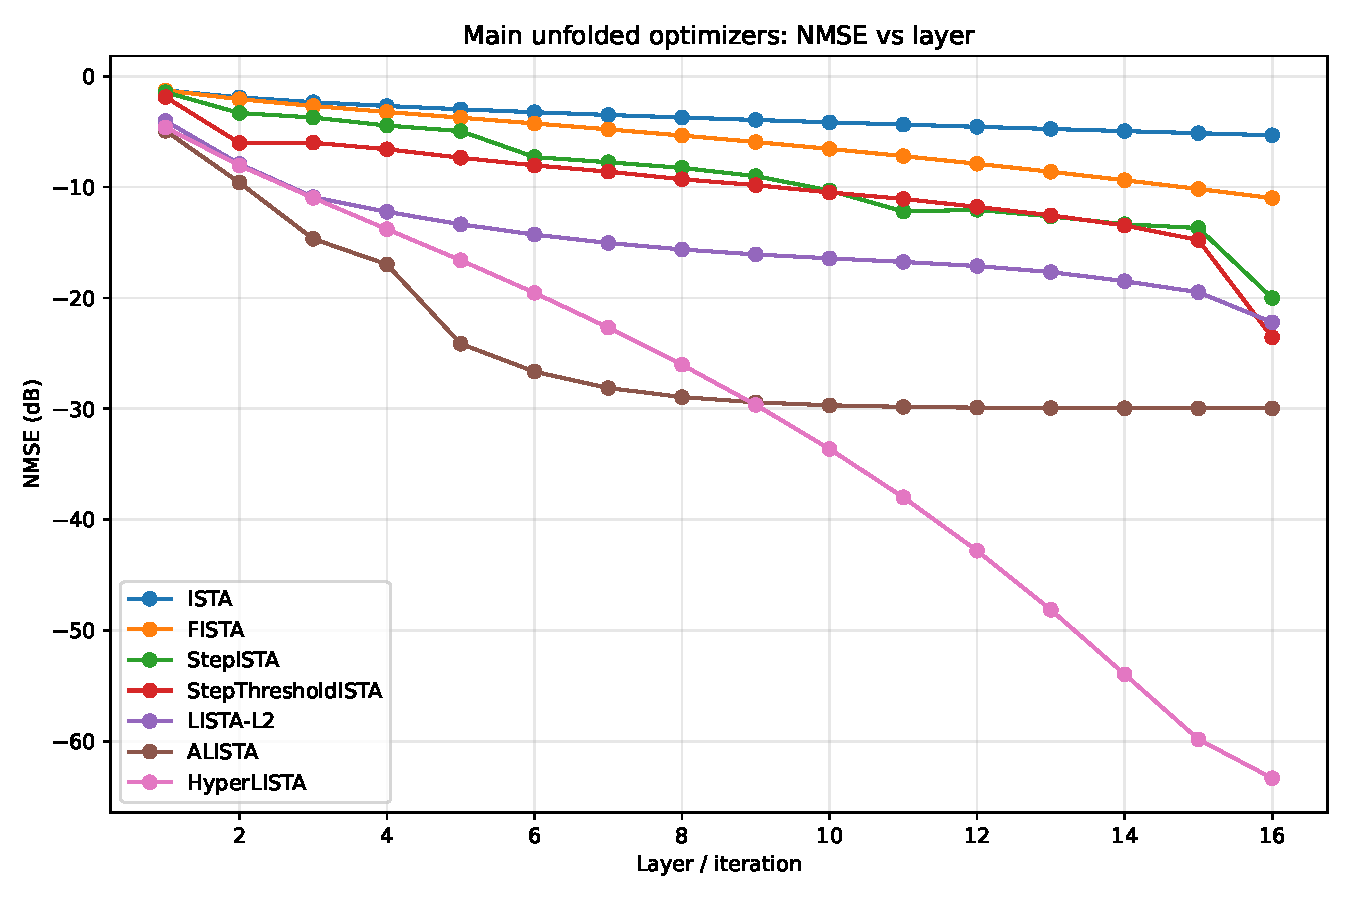
\includegraphics[width=0.62\textwidth]{notebook_03/figures/main_models_nmse_vs_layers.pdf}
\caption{NMSE versus unfolded layer for the main models (Part A). HyperLISTA converges essentially linearly in depth; ALISTA saturates at $-30$\,dB; learned-matrix models are slower per layer despite vastly more parameters.}
\label{fig:main}
\end{figure}

\paragraph{Which ISTA components are worth learning?}
Figure~\ref{fig:scalar} isolates the contribution of each scalar family. Learning thresholds alone (ThresholdISTA) yields only $+1.8$\,dB over ISTA: with the conservative step $1/L$, the iterates change too slowly for threshold tuning to matter. Learning the \emph{step-size schedule} alone (StepISTA, 16 scalars) is transformative --- $-20$\,dB, on par with 6M-parameter LISTA --- because a learned, aggressive schedule (large early steps, decaying later) compensates for the finite depth. Decoupling the threshold from the step (StepThresholdISTA) adds another $3.6$\,dB at negligible cost. \textbf{The step-size schedule is the bottleneck component; matrix learning is largely redundant when $A$ is fixed.}

\begin{figure}[h]
\centering
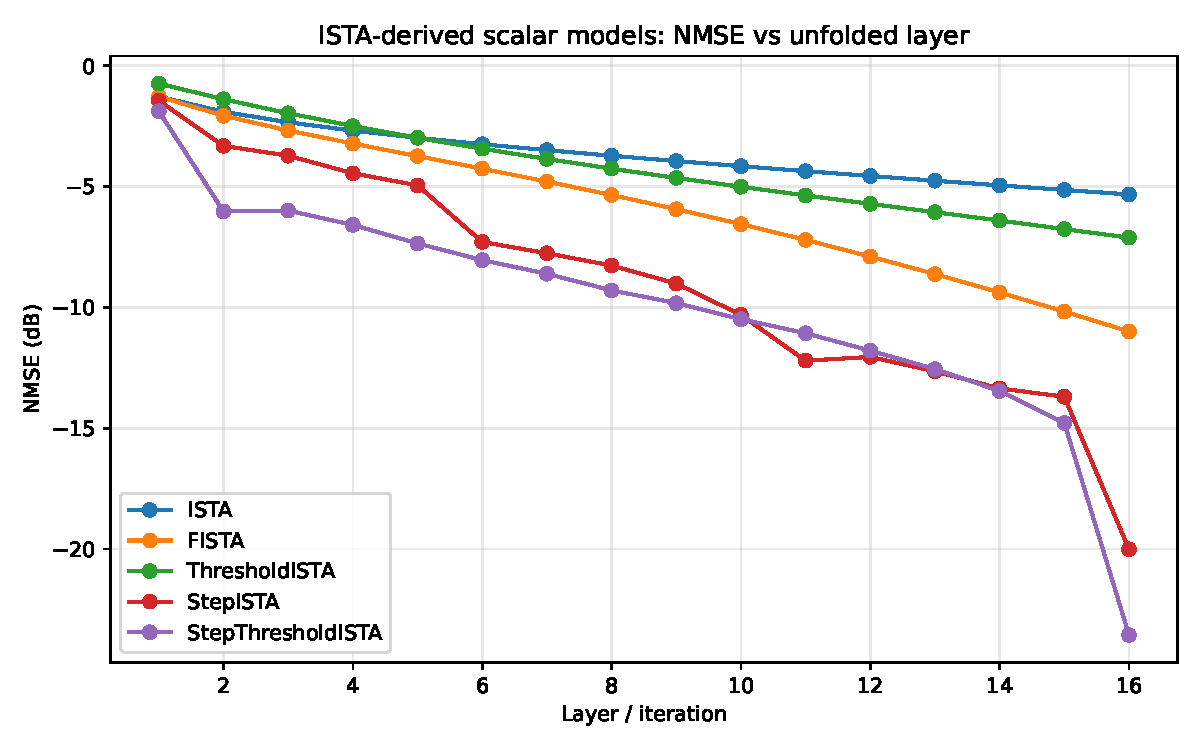
\includegraphics[width=0.55\textwidth]{notebook_03/figures/scalar_ista_variants_nmse_vs_layers.pdf}
\caption{ISTA-derived scalar models (Part A). StepISTA and StepThresholdISTA accelerate sharply in the final layers --- the learned schedule exploits the fixed depth budget.}
\label{fig:scalar}
\end{figure}

\paragraph{Training strategies.}
Deep supervision (L2) is the best training method for untied LISTA ($-21.9$ vs.\ $-20.3$\,dB for L1): intermediate losses stabilize gradients through 16 layers. Greedy layer-wise training (L3) underperforms ($-16.6$\,dB) and its NMSE-versus-layer curve flattens from roughly layer 8 --- each greedy stage optimizes its own output, so later layers have no incentive to improve beyond what earlier layers already achieved. Weight tying loses only $1.2$\,dB relative to untied LISTA while using $16\times$ fewer parameters, acting as implicit regularization.

\subsection{Part B: pixel-domain compressed sensing of real images}

Table~\ref{tab:partB} reports the Fashion-MNIST results at measurement ratio $0.25$, and Figure~\ref{fig:images} shows reconstructions. The ranking \emph{inverts}: the structured methods that dominated Part A now fail --- ALISTA and HyperLISTA fall below plain ISTA --- while LISTA-L2 reconstructs cleanly (SSIM 0.82).

\begin{table}[h]
\centering
\caption{Part B --- Fashion-MNIST pixel-domain CS (ratio $0.25$, $K{=}16$).}
\label{tab:partB}
\begin{tabular}{@{}lrrrr@{}}
\toprule
Method & NMSE [dB] & PSNR [dB] & SSIM & \#Params\\
\midrule
ISTA & $-1.2$ & 8.9 & 0.13 & 0\\
FISTA & $-1.2$ & 8.9 & 0.14 & 0\\
StepThresholdISTA (ours) & $-1.2$ & 8.9 & 0.13 & 32\\
ALISTA & $-0.9$ & 8.4 & 0.12 & 32\\
HyperLISTA & $-0.3$ & 7.7 & 0.09 & 3\\
\textbf{LISTA-L2} & $\mathbf{-13.7}$ & \textbf{22.3} & \textbf{0.82} & 12M\\
\bottomrule
\end{tabular}
\end{table}

The cause is a \emph{signal-model mismatch}. ALISTA's and HyperLISTA's derivations assume i.i.d.\ Gaussian sparse signals with exactly $s$ random non-zeros. Image pixels are bounded in $[0,1]$, non-negative, spatially correlated, and only ``soft-sparse.'' HyperLISTA's residual-driven threshold $\theta^{(k)} = c_1\mu\norm{A^{+}(Ax^{(k)}-b)}_1$, calibrated for sparse Gaussian residuals, instead zeroes out valid image content. LISTA wins precisely because it makes no such assumption --- with $51$K training images it learns the actual pixel distribution.

Sweeping both datasets and both measurement ratios confirms the pattern: on MNIST at ratio $0.5$ (an easy, genuinely sparse task) all methods are reasonable and the structured models degrade gracefully; as the data grow more textured (Fashion-MNIST) and measurements fewer (ratio $0.25$), every prior-based method collapses while LISTA-L2 maintains SSIM $\geq 0.82$ across all four scenarios.

\begin{figure}[h]
\centering
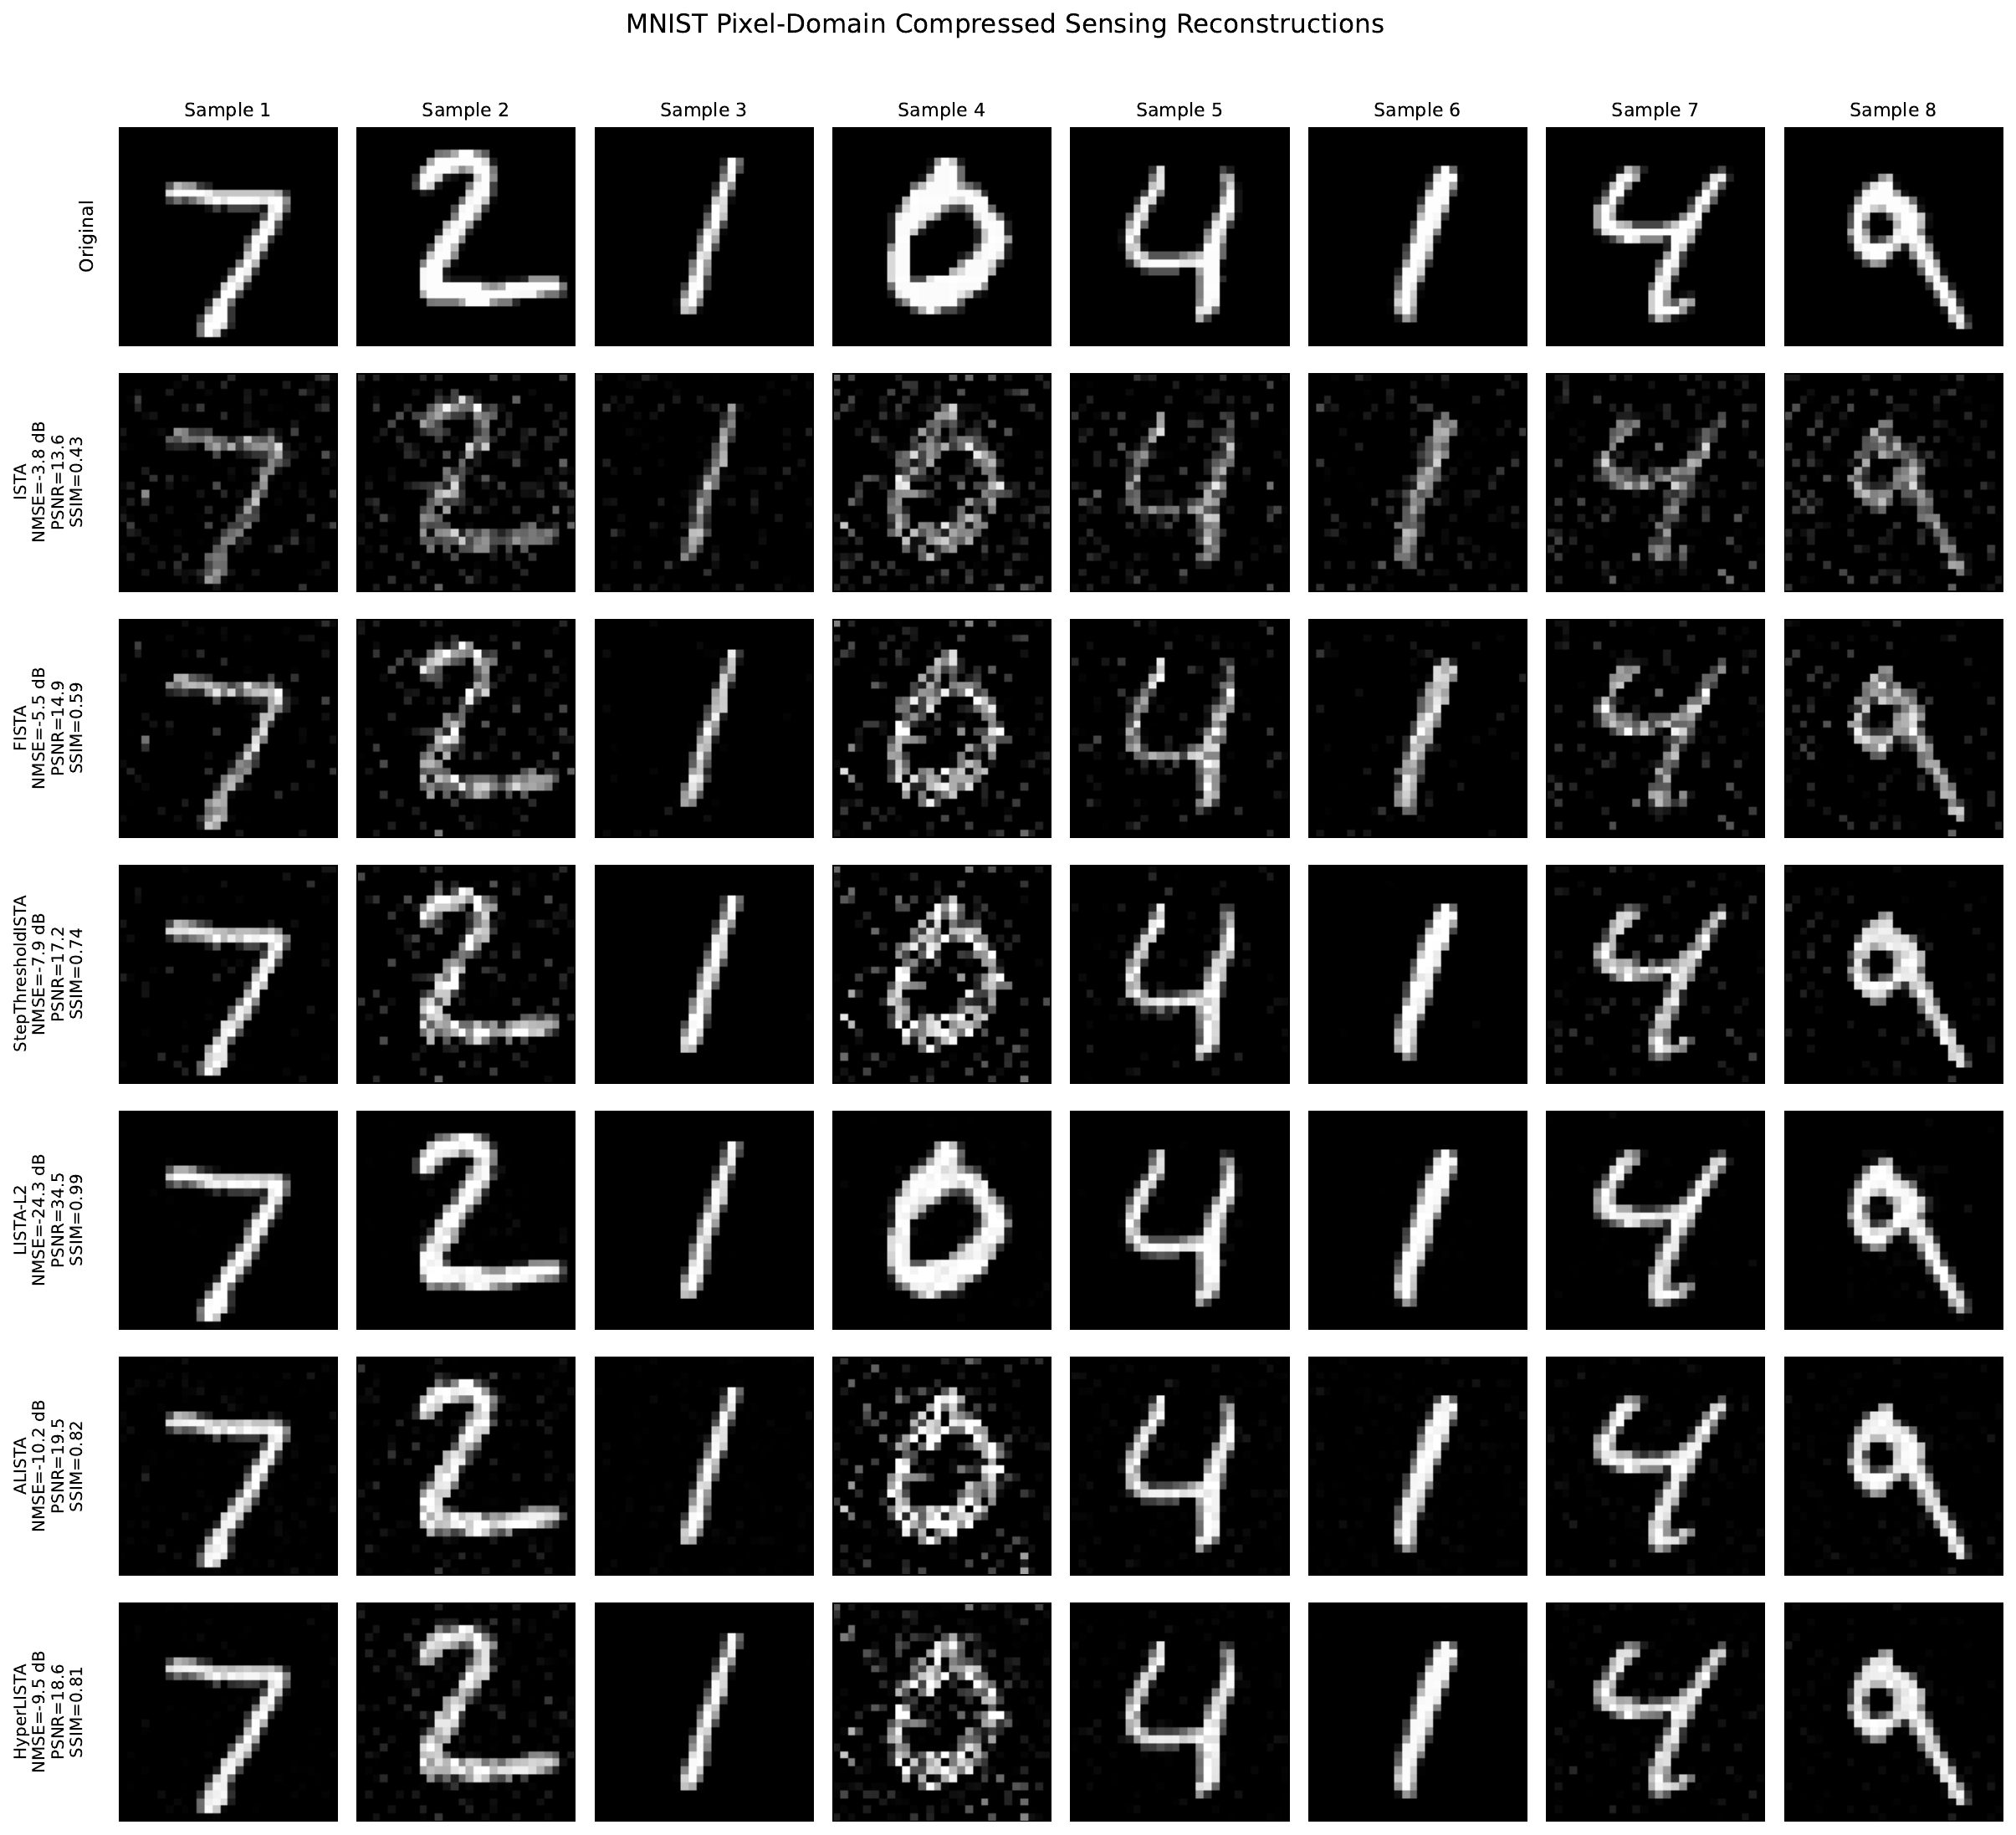
\includegraphics[width=0.49\textwidth]{mnist_grid_025.png}\hfill
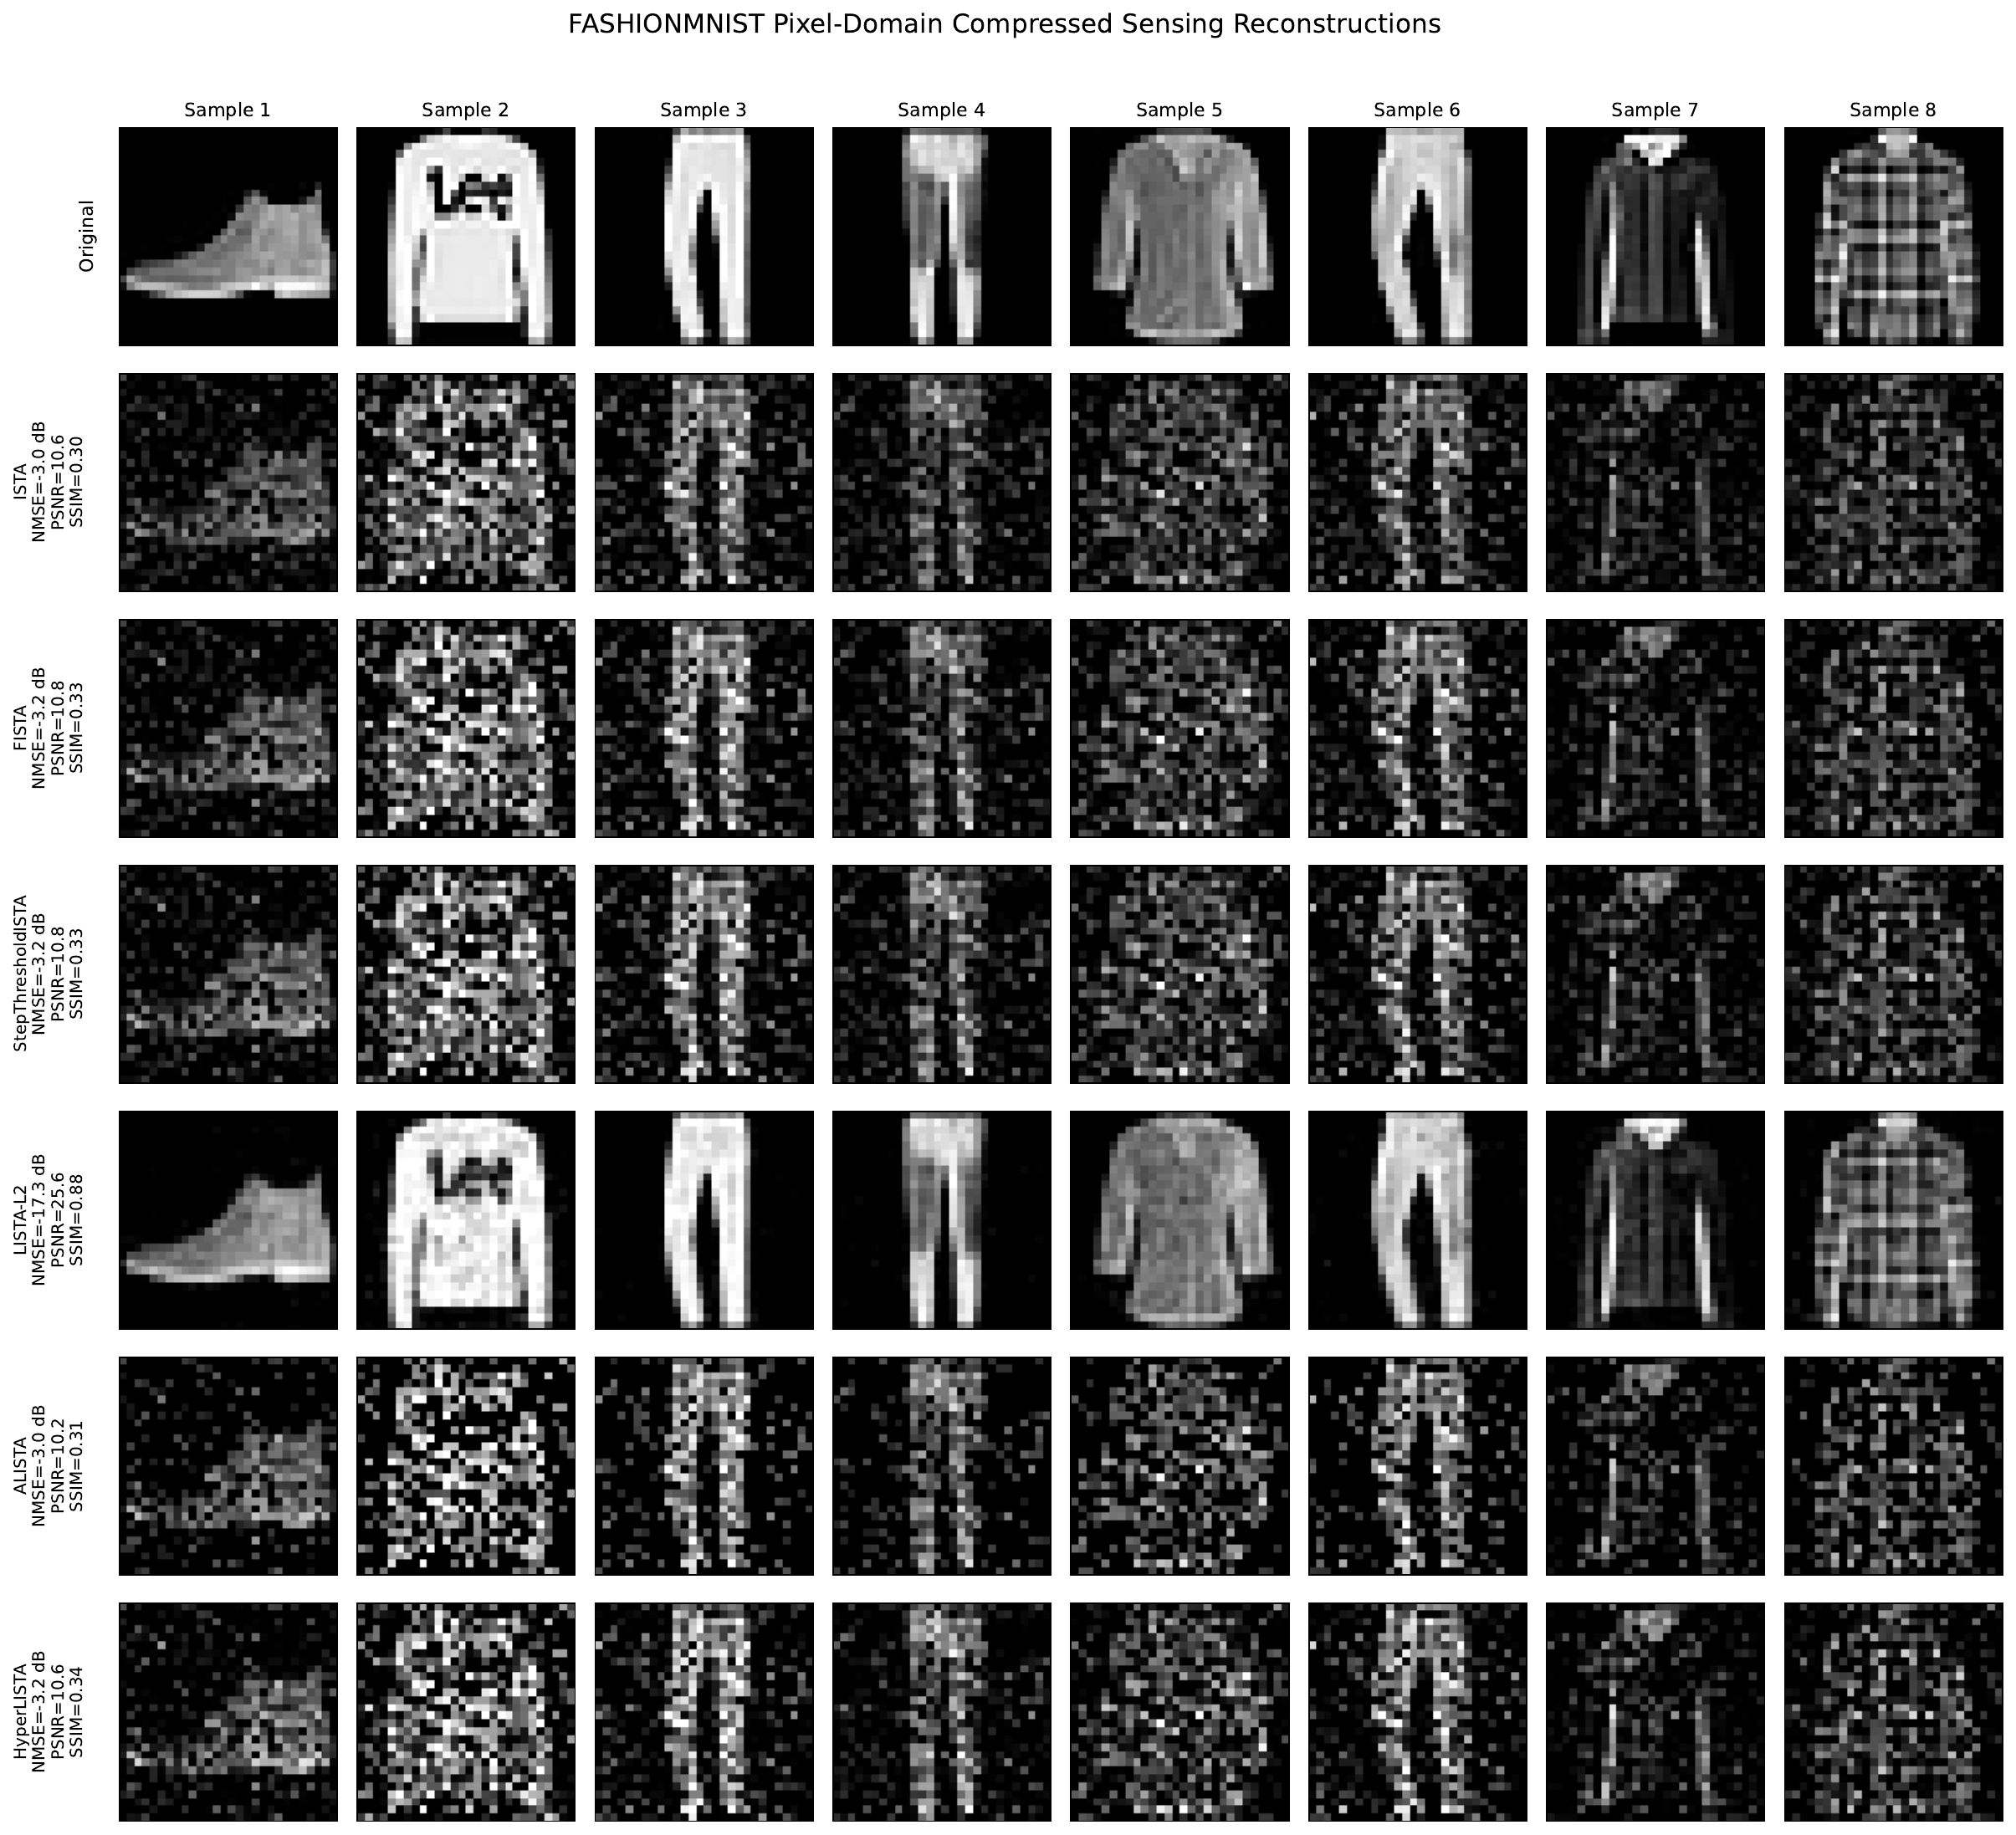
\includegraphics[width=0.49\textwidth]{fmnist_grid_025.png}
\caption{Visual stress test at ratio $0.25$ (left: MNIST, right: Fashion-MNIST; rows: ground truth, ISTA, FISTA, StepThresholdISTA, LISTA-L2, ALISTA, HyperLISTA). LISTA-L2 recovers clean structure on both datasets; the Gaussian-sparse-calibrated thresholds of ALISTA/HyperLISTA erase valid signal on Fashion-MNIST.}
\label{fig:images}
\end{figure}

% ═════════════════════════════ 5. Discussion ════════════════════════════════
\section{Discussion}
\label{sec:discussion}

\paragraph{Bottom line.} In practical terms, our experiments support three operating rules. (i) If the signal truly follows a known sparse model, use a HyperLISTA-style method: three tuned scalars, no gradient training, and the best accuracy by a wide margin. (ii) If the model holds but only a small depth budget is available, learning 16--32 scalars (step sizes, and secondarily thresholds) recovers LISTA-level accuracy at negligible parameter cost --- this is the regime of our StepISTA/StepThresholdISTA designs. (iii) If the signal model is uncertain --- e.g., real images --- prefer a flexible learned model such as LISTA with deep supervision, because model-based shortcuts fail abruptly, not gracefully, under mismatch.

\paragraph{Structure wins when assumptions match.} On data that satisfies the Gaussian-sparse model, adding structure simultaneously removed parameters and improved accuracy, culminating in HyperLISTA's $-61.4$\,dB from 3 grid-searched scalars --- a $41$\,dB advantage over 6M learned parameters. This is the MBDL thesis in its purest form: when the model is right, learning should be confined to the few quantities the theory cannot fix.

\paragraph{The step-size schedule is what matters.} Our ablation localizes the value of learning in unrolled ISTA: 16 learned step sizes recover essentially all of LISTA's gain, while 16 learned thresholds recover almost none. This offers practical guidance for designing unrolled networks under tight parameter budgets --- and explains \emph{why} ALISTA-style architectures work: they keep exactly the components (per-layer $\gamma_k, \theta_k$) that matter.

\paragraph{Wrong prior is worse than no prior.} Part B is deliberately adversarial to the structured methods, and they fail as theory predicts. This is an empirical instance of a point emphasized in the course text \cite{shlezinger2023mbdl}: the statistical models underlying model-based methods are \emph{surrogate approximations} of the true data distribution, and such surrogates ``can be quite unfaithful to the true data'' --- e.g., a Gaussian prior permits negative values that image pixels never take. The practical lesson is not that HyperLISTA is fragile, but that its guarantees are conditional on the signal model; deploying a model-based method requires validating the model. A mismatch does not degrade performance gracefully by default --- an adaptive threshold calibrated to the wrong residual statistics actively deletes signal.

\paragraph{Limitations.} (i) Both parts use a fixed sensing matrix for training and testing; generalization across matrices was not evaluated. (ii) The main comparison is noiseless; preliminary noisy experiments ($\mathrm{SNR}=20$\,dB) preserved the ranking of Part A with reduced margins, but a systematic multi-seed noise study remains future work. (iii) Our HyperLISTA uses batch-median aggregation for $\theta^{(k)}, p^{(k)}$ rather than fully per-sample rules, and its $c_3$ search range had to be widened for images (optimal $c_3\approx 0.01$--$0.17$, far below the synthetic-case range) --- itself evidence of the model mismatch. (iv) Single-seed results; error bars were not computed.

\paragraph{Future work.} The natural continuation is to move the image experiments to a transform domain (DCT/wavelets), where image coefficients are closer to the Gaussian-sparse model and ALISTA/HyperLISTA are expected to partially recover; and to design image-aware thresholding rules for bounded, non-negative signals.

% ═════════════════════════════ References ═══════════════════════════════════
\begin{thebibliography}{9}
\setlength{\itemsep}{2pt}

\bibitem{beck2009fista}
A.~Beck and M.~Teboulle,
``A fast iterative shrinkage-thresholding algorithm for linear inverse problems,''
\emph{SIAM Journal on Imaging Sciences}, vol.~2, no.~1, pp.~183--202, 2009.

\bibitem{gregor2010lista}
K.~Gregor and Y.~LeCun,
``Learning fast approximations of sparse coding,''
in \emph{Proc.\ 27th International Conference on Machine Learning (ICML)}, 2010.

\bibitem{chen2018lista}
X.~Chen, J.~Liu, Z.~Wang, and W.~Yin,
``Theoretical linear convergence of unfolded ISTA and its practical weights and thresholds,''
in \emph{Advances in Neural Information Processing Systems (NeurIPS)}, 2018.

\bibitem{liu2019alista}
J.~Liu, X.~Chen, Z.~Wang, and W.~Yin,
``ALISTA: Analytic weights are as good as learned weights in LISTA,''
in \emph{International Conference on Learning Representations (ICLR)}, 2019.

\bibitem{chen2021hyperlista}
X.~Chen, J.~Liu, Z.~Wang, and W.~Yin,
``Hyperparameter tuning is all you need for LISTA,''
in \emph{Advances in Neural Information Processing Systems (NeurIPS)}, 2021.

\bibitem{shlezinger2023mbdl}
N.~Shlezinger and Y.~C.~Eldar,
``Model-based deep learning,''
\emph{Foundations and Trends in Signal Processing}, vol.~17, no.~4, pp.~291--416, 2023.

\bibitem{lecturenotes}
N.~Shlezinger, \emph{Model-Based Deep Learning (361.2.2320) --- Lecture Notes 1--8},
Ben-Gurion University of the Negev, 2026.

\end{thebibliography}

\end{document}
